% Scoped ICLR submission candidate; full research history is retained separately.
\documentclass{article}
\usepackage{iclr2027_conference,times}
\usepackage{amsmath,amssymb,amsthm,graphicx,booktabs,microtype,xcolor}
\usepackage{etoolbox}
\usepackage[colorlinks=true,linkcolor=blue!55!black,citecolor=green!45!black,urlcolor=blue!70!black]{hyperref}
% Internal draft labels; the shared conference style is unchanged.
\makeatletter
\patchcmd{\@maketitle}{Under review as a conference paper at ICLR 2027}{Submission draft for ICLR 2027}{}{\errmessage{Draft header patch failed}}
\patchcmd{\@maketitle}{Paper under double-blind review}{Anonymous submission draft}{}{\errmessage{Draft title patch failed}}
\makeatother
\newtheorem{proposition}{Proposition}
\newcommand{\HH}{\mathcal H}
\newcommand{\EE}{\mathbb E}
\newcommand{\RR}{\mathbb R}
\title{LatentSpring: Physics-Informed Molecular Flow Matching from Atomic Composition}
\author{Anonymous}
\begin{document}
\maketitle
\begin{abstract}
Generating three-dimensional molecules from atomic composition requires inferring
spatial organization without a supplied chemical graph. We introduce LatentSpring,
a flow-matching framework with a source distribution built from random harmonic
networks over latent trees. Atomic identities and covalent radii determine the
starting spatial structure, while a matrix-tree expression gives its normalized
density after averaging over trees. In matched OMol25 continuations, the harmonic
source raises raw chemical-graph validity by 6.91 percentage points across 64 new
compositions spanning 17--64 atoms. Covariance controls and self-conditioning
ablations identify contributions from mixture structure and provisional-geometry
feedback. The source also improves a separately trained EGNN flow. We derive local physical training targets from forces and transfer
their learned update relative to a matched replay continuation. This improves raw
energy and force under eSEN and independent GFN2-xTB evaluation. A same-norm update
control supports the contribution of the physical update direction. A molecular
rotor experiment verifies complete escorted-work correction against resolved local
target distributions. Generation uses one trained network with 128 evaluations
per sample, without energy-based selection or geometry optimization at inference.
\end{abstract}

\section{Introduction}
Molecular generators must turn an unstructured coordinate distribution into a
configuration compatible with its atoms. The source distribution determines part
of this learning problem: independent Gaussian coordinates carry little molecular
organization, while graph-conditioned harmonic priors encode relationships that
must already be known. This distinction matters when the input specifies atomic
composition and electronic conditions without a chemical graph, as in the
bond-free OMol25 setting considered here.

LatentSpring introduces spatial dependence before learning the transport, while
leaving the final chemical graph unspecified. We sample a latent tree over atoms,
draw Gaussian displacements along its edges at atom-dependent scales, integrate
them into coordinates, and remove translation. Marginalizing the tree defines a
mixture of harmonic networks. The tree is an auxiliary source variable: the neural
field receives coordinates and molecular conditions, and can generate chemical
connectivities different from the sampled source tree. A matrix-tree expression
makes the mixture density explicit.

We integrate this source with equivariant flow matching
\citep{lipman2023flowmatching} and geometry self-conditioning (SC). Controlled comparisons hold the backbone, initialization,
training data, optimization and inference budget fixed while changing the source.
The harmonic mixture improves raw graph validity in both continuations and repeats
its advantage on two subsequent composition panels. Comparing with both a narrower
shell source and an approximate covariance-matched Gaussian distinguishes the
useful source structure from simply imposing near-fixed distances or increasing
second moments.

Physical feedback provides a second way to improve the generator. We construct
local training samples using forces at generated anchors, fit a physical-target
model and a matched replay model, and transfer the difference between their
parameter updates. This brings physical information into the network itself.
For energy reweighting, known local reference densities make the complete
Jarzynski-type work tractable. We test the resulting generator on new compositions
and examine the work correction separately on molecular torsional targets.

Our contributions are: (i) a normalized molecular harmonic-mixture source with
latent spatial connectivity and no supplied bond graph; (ii) its integration with
molecular flow matching and training-only physical feedback; and (iii) controlled
source comparisons, tests on new compositions and evaluation under two energy
models. The generator experiments measure structural validity and energy/force
scores at raw coordinates. The work experiments test distribution recovery against
explicit local reference targets.

\section{Related work}
\paragraph{Molecular flows and source distributions.}
FlowMol3 supplies our equivariant coordinate network \citep{flowmol3}:
rotating its input rotates its predictions, and relabeling identical atoms
relabels the outputs. We reuse its geometry self-conditioning modules.
ET-Flow uses harmonic sources constructed from a supplied molecular graph
\citep{etflow}. More general source adaptation includes guidance under a frozen
field \citep{wang2026sourceguided} and learned conditional sources
\citep{kim2026bettersource}. LatentSpring constructs its molecular source from
atomic composition by integrating over auxiliary spatial trees.

\paragraph{Distributions over trees.}
Factored tree distributions and tractable tree learning provide the probabilistic
basis for our construction \citep{meila2000trees,duan2023spanning}. Gaussian mixtures
over random spanning-tree differences have also been used in imaging inverse
problems \citep{everink2026random}. Here, isotropic edge vectors and atomic length
scales define a density on centered molecular coordinates. Our Gaussian, shell and
covariance controls test which aspects of this structure help the molecular flow.

\paragraph{Physical feedback and nonequilibrium work.}
OMol25 provides molecular structures, energies and forces across electronic
conditions \citep{omol25}. Energy-weighted flow matching \citep{dern2025energyweighted} and target-density
training with importance sampling \citep{fab} incorporate physical information
into generative models. Physical-reward fine-tuning offers a further route for
molecular diffusion models \citep{zhou2025rlpf}. Jarzynski's equality relates
nonequilibrium work to equilibrium free-energy differences; Hummer--Szabo
reconstruction applies it to single-molecule pulling
\citep{jarzynski1997master,hummerszabo2001}. Escorted transport extends this relation
to imposed flow fields with the corresponding volume correction
\citep{escorted2008}. We use normalized local references to specify the physical
training targets and their complete work weights.

\begin{figure}[t]
\centering
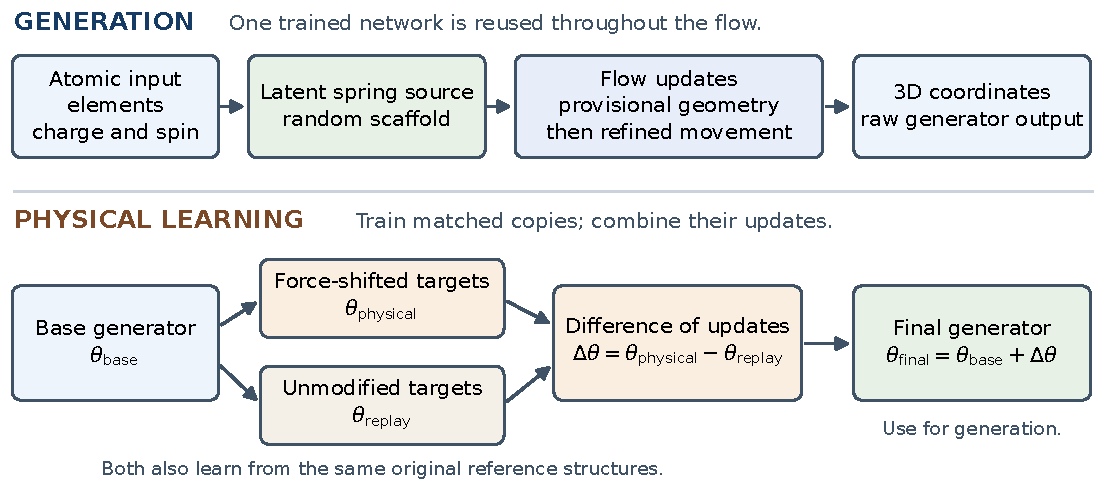
\includegraphics[width=\linewidth]{../research/figures/reader_overview_v1/method.pdf}
\caption{LatentSpring separates generation from physical learning. Top: a
random spring scaffold organizes the starting coordinates, and repeated network
predictions generate the final geometry. Bottom: physical and replay continuations
share their training schedule; their weight difference updates the base generator.
Generation uses the resulting single model.}\label{fig:method}
\end{figure}

\section{A harmonic source with latent connectivity}
The input specifies which atoms are present, their total electrical charge, and
their electronic spin state. It leaves the bonds and positions to be generated.
For example, the composition $\mathrm{C_2H_6O}$ specifies two carbon atoms, six
hydrogens and one oxygen, while allowing different molecular connectivities.
We use $c$ as shorthand for this input: $z_i$ is the atomic number identifying
the element of atom $i$, $Q$ is the net charge in elementary-charge units, and
$S$ is the spin multiplicity. A neutral singlet has $Q=0$ and $S=1$.

There are $N$ atoms. Their positions form a matrix $X\in\RR^{N\times3}$ whose
row $x_i$ contains the three coordinates of atom $i$, measured in angstroms.
We subtract their mean position because the molecule's absolute location is
arbitrary. We denote the resulting centered coordinate space by
$\HH_N=\{X:\sum_i x_i=0\}$; it has $3(N-1)$ independent coordinates.

\paragraph{A random scaffold for the starting coordinates.}
We first connect the atoms by an auxiliary spanning tree $T$: a connected graph
with $N-1$ edges and no cycles. Its edges organize the starting cloud and do not
specify the final chemical bonds. Each possible edge $(i,j)$ receives a positive
weight $a_{ij}=a_{ji}$, called its affinity. A tree's probability is proportional
to the product of its edge affinities:
\begin{equation}
 p(T\mid c)=\frac{\prod_{(i,j)\in T}a_{ij}}{\tau(a)},\qquad
 \tau(a)=\sum_{T\text{ spanning tree}}\prod_{(i,j)\in T}a_{ij}.
 \label{eq:tree-law}
\end{equation}
Here $\tau(a)$ sums those products over all spanning trees, making their
probabilities sum to one. We use factorized affinities $a_{ij}=u_i u_j$, with
$u_i=0.05$ for H and
F/Cl/Br/I, and otherwise $u_i=\max(1,\text{default valence}(z_i)-1)$.
The scalar $u_i$ controls how readily atom $i$ appears in tree edges. These
settings favor fewer connections for hydrogen and halogens, which usually occupy
terminal positions. Default valence is the element's tabulated bonding capacity, counting bond order;
no molecule-specific bonds are supplied.

\paragraph{Gaussian edge laws and sampling.}
For each tree edge, we draw a random three-dimensional displacement between its
atoms. The characteristic length $\ell_{ij}$ is the sum of their covalent radii,
which estimates a typical single-bond separation. Set
$\sigma_{ij}^2=\ell_{ij}^2\exp(s^2)/3$, with $s=0.2$ fixed throughout.
The displacement $d\in\RR^3$ has probability density
\begin{equation}
 h_{ij}(d)=(2\pi\sigma_{ij}^2)^{-3/2}
 \exp\!\left[-\frac{\|d\|^2}{2\sigma_{ij}^2}\right].
 \label{eq:edge-law}
\end{equation}
Here $\|d\|$ is its Euclidean length and $\sigma_{ij}$ is the standard deviation
along each coordinate axis. All directions are equally likely; the radius-based
scale sets the typical separation. This scale also matches the edge covariance
of the lognormal shell control. We sample
a tree with the weighted Wilson algorithm, draw its independent edge vectors,
place atoms by adding these vectors along tree paths, and subtract the coordinate
mean. A new tree is drawn for each sample. Rotating the molecule or relabeling
identical atoms leaves this probability law unchanged.

\paragraph{The distribution after averaging over trees.}
The source density $q_0(X\mid c)$ describes the probability of starting coordinates
$X$ given the atomic input $c$. Averaging over the unobserved tree gives a mixture
of harmonic networks:
\begin{proposition}[Normalized source density]
For normalized isotropic edge densities,
\begin{equation}
 q_0(X\mid c)=N^{3/2}
 \frac{\tau\big(a_{ij}h_{ij}(x_i-x_j)\big)}{\tau(a)}
 \label{eq:source}
\end{equation}
integrates to one over the centered coordinate space $\HH_N$.
\end{proposition}
In the numerator, each affinity is multiplied by the density of its observed
edge displacement. The factor $N^{3/2}$ accounts for expressing independent edge
vectors as centered atomic coordinates. The matrix-tree theorem evaluates each
tree sum as a matrix determinant, avoiding enumeration of all trees. The normalizing factor is derived in Appendix~\ref{app:proof}.

The term \emph{harmonic} refers to the quadratic spring energy associated with
each Gaussian edge law. These virtual springs define a spatially organized random
starting distribution. The learned flow establishes the final molecular geometry.

\section{Integration with molecular flow matching}\label{sec:flow}
Flow matching learns how to move a random starting structure toward a training
structure. We draw starting coordinates $X_0$ from the harmonic source and take
reference coordinates $X_1$ from OMol25. Before pairing them, we match atoms of the
same type and rotate the structures to shorten their coordinate displacement.
We then apply a shared random rotation, uniform over orientations, and a shared
random relabeling of identical atoms. This preserves the source distribution
(Appendix~\ref{app:symmetry}).

The interpolation coordinate $t\in[0,1]$ describes progress from the source
($t=0$) to the reference ($t=1$), rather than physical simulation time.
The training path is $X_t=(1-t)X_0+tX_1$. Its velocity is the constant matrix
$V^*=X_1-X_0$, giving a supervised target for each atom's movement.

\paragraph{Predicting with a provisional geometry.}
The neural network's trainable weights are denoted by $\theta$. Its coordinate
output is $D_\theta(X_t,t)$, which we convert to velocity as
$v_\theta=D_\theta-X_t$. Geometry self-conditioning means giving the network its
own provisional endpoint as an additional input. A first evaluation predicts
velocity $v^{(0)}$, yielding the endpoint estimate
$\widehat X_1=X_t+(1-t)v^{(0)}$. The factor $1-t$ is the remaining interpolation
interval. A second evaluation uses this estimated geometry to predict a refined
velocity $v^{(1)}$. Both evaluations share network weights.

We supervise both predictions so that the provisional geometry also learns from
the reference displacement. Their mean squared velocity error is
\begin{equation}
 \mathcal L_{\rm FM}=\frac12\EE\left[
 \frac{\|v^{(0)}-V^*\|_F^2+\|v^{(1)}-V^*\|_F^2}{3N}\right].
\end{equation}
The expectation $\EE$ averages over training structures, source draws and random
values of $t$. The squared Frobenius norm $\|\cdot\|_F^2$ sums errors over all
$3N$ coordinate components; dividing by $3N$ gives equal weight to each molecule.
The factor $1/2$ averages the two predictions. Gradients pass through both
evaluations. Atomic categories and charge inputs remain fixed, and edge inputs carry a
constant no-bond state. The FlowMol3 source comparisons share this coordinate-only
objective and the same two-pass self-conditioning architecture.

Generation repeatedly follows the learned velocity toward $t=1$. We use 32
midpoint integration steps: each evaluates the velocity at the start and midpoint
of an interval. Two self-conditioning passes per velocity evaluation give
$32\times2\times2=128$ primitive network evaluations per attempted sample, followed
by 0.025\,\AA\ centered Gaussian noise. The FlowMol3 source comparisons use this same
sampler. We evaluate its raw coordinates directly, without subsequent energy
selection or geometry optimization.

\subsection{Physical feedback through paired training targets}
Physical learning uses energy and force information during training to improve
the coordinates produced by the final network. A frozen harmonic generator first
produces training structures, called anchors and denoted by $A$, on compositions
excluded from evaluation. For each anchor that passes the chemical-graph checks,
we draw nearby coordinates from a small centered Gaussian cloud
$q_A=\mathcal N_{\HH_N}(A,\sigma_A^2I)$. Here $\sigma_A$ sets the size of local
perturbations and $I$ is the identity covariance on the centered space.

The teacher uses the learned eSEN energy model, with energy $E_+$ and force $F_+$,
averaged over mirror-related coordinates to enforce reflection symmetry
(Appendix~\ref{app:local-work}). Locally linearizing this energy shows that
Boltzmann weighting shifts the Gaussian's mean by
$\delta_A=\sigma_A^2F_+(A)/(k_B T_{\rm phys})$, where $k_B$ is Boltzmann's
constant and $T_{\rm phys}=300$ K is the teacher temperature.
Applying this displacement to each nearby structure gives $Y=X+\delta_A$,
called a force escort. We choose the perturbation scale to bound the displacement,
and fix both quantities before drawing candidates. Appendix~\ref{app:local-work}
derives this local Boltzmann approximation and specifies its geometric restriction.

The already-trained harmonic generator has weights $\theta_{\rm base}$.
We make two copies of these weights. The physical copy learns
from the force-shifted targets and produces $\theta_{\rm physical}$. The replay
copy follows the same training schedule using the original generated anchors,
producing $\theta_{\rm replay}$. Both copies also receive the same updates
on original OMol25 references. Replay measures the change caused by refitting
generated structures without their physical displacement. We construct the final
network weights by adding the difference between these continuations to the
original model:
\begin{equation}
 \theta_{\rm final} = \theta_{\rm base} + (\theta_{\rm physical}-\theta_{\rm replay}).
 \label{eq:physical-transfer}
\end{equation}
The subtraction defines a physical-versus-replay update direction. Its addition
to $\theta_{\rm base}$ is parameter arithmetic \citep{ilharco2023arithmetic}, applied
elementwise to matching weight tensors with coefficient one. The result is one
neural generator; the two training copies are not evaluated during generation.
Direct and
paired-update results are reported in Appendix~\ref{app:local-work}.

\paragraph{Correcting the distribution of local candidates.}
Complete escorted-work weighting \citep{escorted2008} provides a local extension
that favors lower-energy structures while retaining the Gaussian restraint around
each anchor. Because the escort changes where candidates are sampled, energy
differences alone do not give the target weights. For candidates retaining the
anchor's inferred connectivity, define
\begin{equation}
 W_A=E_+(Y)-E_+(A)+k_B T_{\rm phys}[\log q_A(X)-\log q_A(Y)].
 \label{eq:main-local-work}
\end{equation}
The work $W_A$ has energy units. Its first term measures the energy change;
the logarithmic density ratio corrects the sampling shift.
The map is a fixed translation, so its volume-change factor is one.
Weights $\exp[-W_A/(k_B T_{\rm phys})]$ estimate the local target's normalizing
constant and determine how often each candidate is used for training. We compare
uniform and complete-work training weights, and use the
less expensive force update as the primary candidate for the new-composition
physical evaluation. Appendix~\ref{app:local-work} gives the target definition,
particle construction and training controls.

\section{Experimental design}
\paragraph{Task and training.}
We study adaptation of a pretrained molecular flow to coordinate generation from
neutral singlet organic compositions. Each composition contains C and H and uses
elements from H/B/C/N/O/F/Si/P/S/Cl/Br/I. Source-model training covers 8--40 atoms; evaluation extends to 64 atoms. The
implementation supports up to 200. Two continuations start from a shared pretrained
checkpoint. Each uses 3,000 distinct OMol25 structures and 3,000 optimizer updates,
with identical data and initialization across its source variants. The vector
field has 5,904,369 parameters. The backbone learning rate is $2\cdot10^{-5}$ and
the self-conditioning modules use $3\cdot10^{-4}$.

Training structures pass the graph assay and a geometric filter requiring a
bounded-edge, degree-capped scaffold. This filter is specified in the data-selection
protocol. The models receive the selected coordinates; the scaffold is used for
selection only. All source variants use the same filtered subset.

\paragraph{Composition panels.}
The source studies use 12 development compositions, ten additional compositions,
24 fresh compositions and a broader 64-composition panel. The latter three are
absent from both processed OMol25 corpora by exact atomic-count checks. Reference
coordinates qualify the evaluation conditions and are excluded from fitting.
The pretrained studies reuse the same two fitted continuations; the independent
EGNN study trains two new initializations. Selection details and source controls
are given in Appendix~\ref{app:source-panels}.

\paragraph{Metrics and uncertainty.}
The first two panels use 64 samples per composition and the 24-composition test
uses 32. Geometric validity requires a connected contact graph and no short-distance
overlap, with thresholds of 1.25 and 0.6 times the summed covalent radii. Graph
support additionally requires RDKit to construct a connected, sanitized graph
with the specified total charge. We report
support per attempted output, including failed samples and validator exceptions
in the denominator. Distinct perceived connectivities within each composition
measure graph diversity; timings record the full generation procedure.
Appendix~\ref{app:data-evaluation} gives the selection and perception settings.

Unless stated otherwise, 95\% confidence intervals use paired bootstrap resampling
of generation draws, holding the fitted models and compositions fixed. We also
bootstrap compositions to describe variation across the evaluation panel. Physical
scores are computed at the saved raw coordinates using the declared electronic
conditions and approximate potentials.

\section{Results}
\subsection{Effect of the latent spring source}
With backbone, initialization and training data matched, harmonic sources improve
chemical-graph validity over isotropic Gaussian sources by 5.86 percentage points
on 12 development compositions, 8.83 points on ten additional compositions, and
8.20 points on the 24-composition panel below. A Gaussian with approximately
matched covariance also performs worse, supporting a contribution from mixture
structure beyond the tested second-moment approximation. Appendix~\ref{app:source-panels}
reports the detailed source, shell and covariance controls.

\subsection{Generalization across molecular sizes}\label{sec:wide}
We evaluate the frozen source models on 64 further compositions, with 16 in each
of four size ranges from 17 to 64 atoms. All are absent from both processed OMol25
corpora and from the earlier generation panels. The models receive no additional
training. Metadata ranks select each composition after the same reference-validity
checks, with 32 draws per composition and model continuation.

\begin{table}[t]
\centering
\caption{Raw chemical-graph validity on the 64-composition panel. Each size range
contains 1,024 attempts per method across two continuations. Values are percentages;
the final column reports percentage-point differences.}
\begin{tabular}{lrrr}
\toprule
Atoms & Gaussian & Harmonic & Difference\\
\midrule
17--28 & 49.12 & 55.08 & +5.96\\
29--40 & 24.02 & 38.28 & +14.26\\
41--52 & 16.50 & 21.29 & +4.79\\
53--64 & 9.77 & 12.40 & +2.64\\
\midrule
All 64 compositions &24.85&31.76&+6.91\\
\bottomrule
\end{tabular}\label{tab:wide}
\end{table}

The harmonic source improves the pooled rate in every size range. Overall it
adds 6.91 percentage points, with a size-stratified composition-bootstrap 95\%
interval of [4.74,9.03]. The two continuations improve by 11.18 and 2.64 points,
respectively. Absolute validity decreases for larger molecules, while the source
advantage remains positive in the aggregate. These results extend the source
comparison beyond the original 17--28-atom confirmation range.


\subsection{Independent backbone and generator objectives}\label{sec:matched-generators}
Gaussian FM, harmonic FM, position-conditional EDM, and GAGA \citep{edm,qu2026gaga} train from scratch on the same EGNN and 20,000 OMol25 structures. Two repetitions share initialization within each comparison, with 30,000 updates at batch size 32. Neither self-conditioning nor physical adaptation is used. The FM models differ only in source, sharing interpolation and atom pairing (Appendix~\ref{app:matched-generators}).

Harmonic improves FM graph validity by 1.34 points (composition 95\% interval [0.12,2.52]). EDM and GAGA achieve higher validity in this setting, with different paths, objectives, and samplers. Distance self-conditioning subsequently supplies the FM parent for physical-head comparisons at matched training-forward budgets (Appendices~\ref{app:feedback-transfer} and~\ref{app:matched-connection}).

A separate 16-composition complete-system comparison gives 38.87\% GFN2 joint yield for the inherited 5.90-million-parameter FlowMol backbone and 46.88\% with force correction. The 2.38-million-parameter GAGA trained from scratch gives 9.77\% at 128 calls and 12.11\% at 651. Appendix~\ref{app:common-models} details the differing training histories and physical supervision, costs, capacity controls, and fitting-duration study.


\subsection{Fresh composition and cross-potential confirmation}\label{sec:fresh-physics}
After the earlier source and physics studies, we freeze the Gaussian model,
LatentSpring's harmonic model, and both fixed-coefficient physics-update variants.
The cheaper unweighted-force update is designated the primary physical candidate
before querying new outcomes. We sample a new pool of 256 distinct compositions
from the original development partition, excluding every old official candidate
composition. Reference qualification accepts 121; fixed metadata ranks select
8 per 17--20, 21--24 and 25--28 atom bin, yielding 24 new compositions. All selected
compositions are absent from both verified processed corpora. The reference
coordinates do not enter generation or fitting. Every model generates 32 samples
per composition in each of the same two existing continuations: 6,144 new outputs,
with no additional model fitting or parameter selection. Inference uses the
network alone: no per-output energy ranking or coordinate optimization is applied.

\begin{table}[t]
\centering
\caption{Fresh 24-composition graph support, 768 attempts per continuation.
All rates describe raw outputs before any structural relaxation. All methods use
128 primitive denoiser calls per attempted output.}
\begin{tabular}{lrrr}
\toprule
Model & Continuation 1 & Continuation 2 & Pooled rate\\
\midrule
Gaussian reference &332&352&44.53\%\\
LatentSpring harmonic &435&375&52.73\%\\
With force update &439&382&53.45\%\\
With complete-work update &426&383&52.67\%\\
\bottomrule
\end{tabular}\label{tab:fresh-graph}
\end{table}

The harmonic source improves graph support over Gaussian by 8.20 percentage points,
with conditional paired 95\% interval $[5.08,11.33]$. Both continuation signs are
positive. The primary force update has an observed graph-rate difference of
$+0.72$ points versus harmonic, with interval $[-0.98,2.34]$. This is compatible
with unchanged validity and excludes a decline exceeding two points under this
conditional interval; it is not evidence of a statistically significant validity
increase or a population-wide noninferiority guarantee. All accepted graphs have
distinct perceived connectivity within each composition in these draws.

\paragraph{Independent physical readout.}
We evaluate every generated coordinate set with eSEN and with gas-phase GFN2-xTB
single points and analytic gradients \citep{gfn2xtb}. GFN2 is not used for training
or method selection. It provides a different approximate physical model, not
DFT ground truth. We retain all failed calculations: 4 of 6,144 generated-geometry
GFN2 calculations fail, all outside graph support. Every graph-supported output
succeeds, and all original-reference inversion checks pass. Total physical cost
is 12,384 raw eSEN queries and 6,240 GFN2 attempts, including reference checks.
The audited eSEN readout uses $E_+(X)=[E(X)+E(-X)]/2$ and
$F_+(X)=[F(X)-F(-X)]/2$; force RMS is the root mean squared atom-force norm.
GFN2 inputs are fixed at their saved generated coordinates.
The xTB command uses \texttt{--grad}, never \texttt{--opt}; gradients are readouts
and do not update coordinates. Physical teacher displacements occur only in the
earlier training procedure, on separate FIT samples.

\begin{table}[t]
\centering
\caption{Primary force-update change versus the frozen harmonic model on paired
common-graph support. Both continuation signs improve for both readouts under
both potentials. Intervals are conditional paired 95\% intervals.}
\small
\setlength{\tabcolsep}{4pt}
\begin{tabular}{lrr}
\toprule
Potential & Energy change (eV/atom) & Force-RMS change (eV/\AA)\\
\midrule
eSEN & $-0.01308\;[-0.01805,-0.00817]$ & $-0.34793\;[-0.41498,-0.28478]$\\
GFN2 & $-0.01168\;[-0.01616,-0.00724]$ & $-0.35620\;[-0.42983,-0.28714]$\\
\bottomrule
\end{tabular}\label{tab:fresh-physical}
\end{table}

All 24 composition cells in each continuation have comparable graph-supported
pairs for the primary contrast. The prespecified cross-potential confirmation
gate passes, including success coverage and the observed two-point validity
criterion. All-attempt eSEN and common-success GFN2 comparisons agree in direction;
selected-support results remain distinct from unconditional or equilibrium
expectations. Source-only harmonic-versus-Gaussian energy improvements are pooled
positive but heterogeneous across continuations, so we do not describe them as
repeated physical-quality gains in both models.

Complete-work versus force-update energy differences remain unresolved:
$-0.00413$ eV/atom under eSEN, interval $[-0.00903,0.00078]$, and $-0.00363$ under
GFN2, interval $[-0.00792,0.00075]$, on common graph support. Force and graph
intervals also span zero. Thus the fresh result supports the practical physical
feedback update, while not establishing an extra advantage of Jarzynski weighting.
The previously defined local work identity remains mathematically useful, but
these results do not imply globally Boltzmann-distributed generator outputs.



\subsection{What self-conditioning contributes}\label{sec:sc-ablation}
To test the provisional-geometry feedback, we train the harmonic-source model
with self-conditioning removed. Initialization, the 3,000 training structures,
source law and pairing are unchanged. One readout uses 3,000 optimizer updates;
a second uses 6,000, matching the self-conditioned model's number of backbone
training evaluations. A single-pass model takes 64 midpoint steps, so all methods
use 128 network evaluations at generation.

\begin{table}[t]
\centering
\caption{Self-conditioning ablation on the 24-composition panel. Each continuation
has 768 raw attempts; the two counts give continuations 1 and 2. The full model
improves over both single-pass budgets.}
\begin{tabular}{lrrrr}
\toprule
Model & Updates & Training passes & Valid outputs & Rate (\%)\\
\midrule
Single pass &3,000&3,000&363;336&45.51\\
Single pass &6,000&6,000&277;342&40.30\\
Self-conditioned &3,000&6,000&435;375&52.73\\
\bottomrule
\end{tabular}\label{tab:sc-ablation}
\end{table}

Self-conditioning adds 7.23 percentage points at equal optimizer updates
(95\% interval [4.69,9.77]) and 12.43 at equal training-pass count
([9.70,15.23]). Both continuations improve under both comparisons. Matching pass
counts does not equate every operation or wall-clock cost; the comparison tests
whether additional single-pass training recovers the observed validity gain.

The update-direction control appears in Section~\ref{sec:update-ablation}.

\paragraph{Contribution of the force displacement.}
We also remove only the displacement from the local training targets, retaining
the same Gaussian perturbations, candidate indices, widths, training schedule and
paired parameter update. Compared with this control, the force-shifted targets
lower energy by $0.01939$ eV/atom (95\% interval [-0.02417,-0.01455] for the signed
difference) and force RMS by $0.3926$ eV/\AA\ ([-0.4696,-0.3263]) among jointly
valid outputs. Both continuations improve. Graph validity is similar: the
force-minus-control difference is $+0.39$ points with interval [-1.33,2.19].
The original force-dependent widths and candidate-selection rule remain fixed,
so this comparison identifies the contribution of the displacement itself.


\subsection{Complete-work correction on molecular rotors}\label{sec:rotor-work}
To test the work correction directly, we select three methyl rotors from training
molecules in fixed data order, using geometry alone.
Each rotor turns the three hydrogens of a methyl group around its bond axis while
holding the other internal coordinates fixed. The rotation angle $\phi$ therefore
specifies a one-dimensional family of three-dimensional molecular structures.
A periodic interpolant of 512 GFN2 energies supplies their potential $U(\phi)$;
$U(0)$ is the reference energy at angle zero. The target is
$\rho(\phi)\propto q_0(\phi)\exp[-(U(\phi)-U(0))/kT]$, where $q_0$ is a normalized
von Mises reference of concentration one: a smooth circular distribution favoring
angles near zero. The product retains this reference restraint and gives greater
weight to lower-energy angles. Here $kT=k_B T_{\rm phys}$ at 300 K.

Starting from $\phi\sim q_0$, use escorts $\psi_a(\phi)=\phi+a\sin\phi$ for
$a\in\{-0.5,0,0.5\}$. Their positive Jacobian is $J_a=1+a\cos\phi$.
The map $\psi_a$ changes the sampled angle; $a$ sets its strength, and $J_a$
measures how it locally expands or compresses angular intervals. The complete
generalized work includes both reference densities and $-kT\log J_a$
(Appendix~\ref{app:rotor-work}). We compare complete work, energy-only weights,
weights omitting the Jacobian, and unweighted endpoints, with shared draws and
128 repetitions at each of 8, 32, 128, 512 and 2,048 samples.

\begin{figure}[t]
\centering
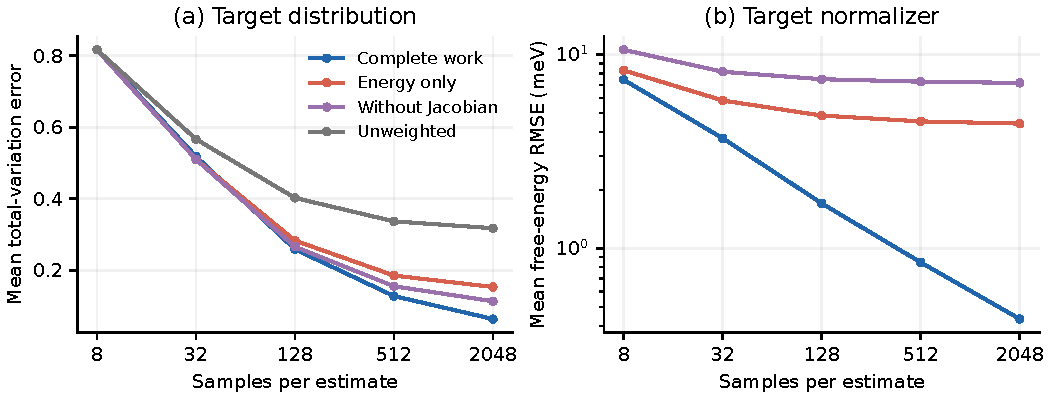
\includegraphics[width=\linewidth]{../research/figures/rotor_work_v1/rotor_work.pdf}
\caption{Complete work corrects the nonequilibrium sampling bias on the specified
torsional targets. Curves average all three molecules and both nonidentity
escorts; each case has 128 repetitions. Energy-only and incomplete-work controls
retain bias as sampling increases. Unweighted endpoints have no free-energy
estimator. Each target is a constrained molecular rotor at 300 K.}\label{fig:rotor-work}
\end{figure}

Total variation measures disagreement between the estimated and target angular
probabilities, with zero indicating agreement. Free-energy RMSE measures error in
the logarithm of the target normalizer, expressed in energy units.

At 2,048 samples, complete work has lower mean total-variation error than both
incomplete-weight controls in all six nonidentity cases. Across these cases,
mean errors are 0.0636 for complete work, 0.1532 for energy-only weights and
0.1134 without the Jacobian, a 58.5\% reduction relative to energy-only weighting.
Complete-work free-energy RMSE ranges from 0.158 to 0.734 meV. Independent
density-ratio quadrature also recovers the specified target normalizer in all
nine molecule/escort cases. The identity-escort control makes the three weighted
methods coincide. Together, the distribution and normalizer results show the
role of complete work accounting on these molecular energy curves.


\section{Discussion}
LatentSpring organizes the starting distribution through latent connectivity and
transfers local physical information into a single molecular flow. Controlled
comparisons support the source, geometry feedback and physical-update choices.
The evidence covers neutral organic compositions, two pretrained-model
continuations and two independent EGNN initializations; intervals condition on
these fitted models. Chemical-graph validity measures structure, energy and force
readouts use approximate potentials, and the work experiments address specified
local ensembles. Broader chemistry and recovery of full molecular equilibrium
remain open directions.

\label{endofmaintext}
\subsubsection*{Reproducibility statement}
The project includes code, model configurations and data-selection manifests.
These specify random seeds, checkpoint hashes, evaluation settings and every
attempted output. We report training, physical preparation and generation costs
separately, and provide tests for source normalization, symmetry, density gradients
and work identities. Source data and pretrained backbones retain their original
licenses and access requirements.

\subsubsection*{AI use statement}
OpenAI Codex and Claude Code assisted literature review, hypothesis and experiment
design, mathematical derivation and proof writing, code implementation, data
preprocessing, testing, experimental analysis, and manuscript drafting and editing.

\bibliography{refs,tree_refs}
\bibliographystyle{iclr2027_conference}
\appendix
\section{Notation and evaluation terminology}\label{app:notation}
LatentSpring samples initial coordinates from composition, transports them with a learned flow, and applies geometric and physical endpoint corrections. The table below collects the notation for these stages and the supplementary studies.

\paragraph{Inputs and outputs.}
The condition $c$ fixes atom identities, charge, and spin. In the experiments, charge and multiplicity are fixed at $Q=0$ and $S=1$. At state $X_t$, the network takes $t$ and encoded atom identities and predicts one velocity per atom. Self-conditioning passes a provisional endpoint from the first evaluation to the second. Integrating the corrected field from a random $X_0$ gives $X_{\rm gen}$, with no terminal perturbation in the main FM model. Earlier samplers specify their own terminal-noise settings. Atom identities and electronic conditions are unchanged; bonds are inferred afterward for evaluation.

\begin{table}[htbp]
\centering
\small
\begin{tabular}{p{0.22\linewidth}p{0.71\linewidth}}
\toprule
Symbol & Meaning\\
\midrule
$N$, $z_i$, $Q$, $S$, $c$ & Atom count, atomic numbers, total charge, and spin multiplicity. The condition $c$ collects these inputs.\\
$X$, $x_i$, $\HH_N$ & Atomic coordinate matrix, the position of atom $i$, and
the space where the mean atomic position is zero. Coordinates are in angstroms.\\
$T$, $a_{ij}$, $u_i$ & Auxiliary spatial tree, its edge affinities, and the
atom-dependent factors defining those affinities. These are source variables.\\
$\ell_{ij}$, $\sigma_{ij}$, $h_{ij}$ & Characteristic separation from covalent
radii, Gaussian displacement scale, and the probability density of one edge vector.\\
$\tau(a)$, $q_0(X\mid c)$ & Sum of tree weights and the normalized distribution
of starting coordinates after averaging over trees.\\
$X_0$, $X_1$, $X_t$, $X_{\rm gen}$, $t$ & Starting, reference, intermediate and
returned coordinates; $t$ labels generation progress, not physical time.\\
$V^*$, $v_\theta$ & Supervised flow velocity and the predicted velocity field.\\
$v^{(0)}$, $v^{(1)}$, $\widehat X_1$ & First and second velocity predictions,
and the provisional endpoint passed between them during self-conditioning.\\
$v_{\rm base}$, $H_t$ & Frozen parent velocity after both self-conditioning passes,
and its extrapolated endpoint used to construct physical training targets.\\
$G_\psi$, $g$, $H_g$ & Geometric correction network, its predicted velocity increment,
and the endpoint after that correction.\\
$A_\phi$, $f$, $\eta$ & Physical correction network, its predicted velocity increment,
and the strength applied to that increment.\\
$\EE$, $\|\cdot\|_F^2$ & Average over the specified random draws, and the sum
of squared entries of a coordinate or force matrix.\\
$\theta_{\rm base}$, $\theta_{\rm physical}$,
$\theta_{\rm replay}$, $\theta_{\rm final}$ & Base weights, weights after physical or replay fine-tuning, and the final generation weights.\\
$A$, $q_A$, $\sigma_A$, $\delta_A$ & Generated anchor, local Gaussian reference, perturbation width, and force-guided shift.\\
$E_+$, $F_+$ & Mirror-symmetrized teacher energy and force, in eV and eV/\AA.
The force is the negative coordinate gradient of this energy.\\
$k_B T_{\rm phys}$, $W_A$ & Thermal energy at the teacher temperature and
generalized work used to weight local candidate structures.\\
$\Phi$, $J$, $Z$ & Coordinate map, its local volume-change factor, and a target-density normalizing integral.\\
\bottomrule
\end{tabular}
\caption{Notation for the source, flow, endpoint corrections, and supplementary physical-update studies.}
\end{table}

\paragraph{Evaluation terminology.}
\emph{Contact support} requires a connected contact graph without excessive overlap. \emph{Graph validity} additionally requires a sanitized inferred chemical graph. \emph{Geometry-and-force yield} applies the bond-length, angle, internal-distance, planarity, and radical screen in Appendix~\ref{app:chemical-geometry}, together with force RMS at most 5 eV/\AA. \emph{Joint graph-and-force yield} uses the same force threshold without the stricter geometry screen. In the paired-update studies, \emph{jointly valid} instead denotes a pair of outputs that both pass contact and graph checks. The teacher's \emph{same-graph} restriction preserves an anchor's labeled bonds, formal charges, and radical counts.

Energy differences are compared within composition and reported per atom. Force RMS is $[N^{-1}\sum_{i=1}^N\|F_i\|_2^2]^{1/2}$. It measures residual atomic forces, whereas energy measures preference under the chosen potential and graph validity measures consistency of inferred connectivity.

\section{Data selection and structural evaluation}\label{app:data-evaluation}
Training data are selected in a fixed shuffled order from the processed OMol25
training corpus, excluding the evaluation compositions. The first 3,000 eligible
structures form each continuation's training set. Eligibility requires the atom,
element and electronic-state conditions in Section 5, the structural assay below,
and a geometric scaffold filter.

The scaffold filter considers pairs whose distance divided by the sum of covalent
radii lies strictly between 0.6501 and 1.1999. Kruskal's algorithm constructs a
minimum normalized-distance spanning tree from these pairs, greedily adding
short edges that do not create a cycle. A structure is accepted
if the tree is connected and its degrees are at most 1 for H/F/Cl/Br/I, 4 for
B/C/N/Si, 3 for O, and 6 for P/S. The scaffold is used only to select training
coordinates; the molecular flow uses its own sampled harmonic source.

Structural evaluation uses RDKit 2025.03.2, a toolkit for representing molecules
and checking chemical consistency. After the contact-connectivity and
overlap checks, \texttt{DetermineBonds} assigns bonds at the specified total charge,
with \texttt{covFactor=1.25}, \texttt{useVdw=True},
\texttt{allowChargedFragments=True}, and \texttt{embedChiral=False}.
Its sanitization step checks valence and related graph-consistency rules.
Sanitization must succeed, the assigned formal charges must sum to the specified
charge, and the perceived molecule must have one connected component. Graph
diversity counts canonical SMILES, standardized text encodings of molecular
connectivity, after removing stereochemical tags and explicit
hydrogens. Evaluator errors and unsupported outputs remain in the attempted-sample
denominator.

\paragraph{The 24-composition confirmation panel.}
We next evaluate the frozen Gaussian, harmonic and two physical-update models on
24 new compositions. The force-only update is chosen as the primary physical
candidate before this evaluation. Starting from a pool of 256 distinct compositions
outside the earlier candidate sets, reference qualification accepts 121. Fixed
metadata ranks select eight compositions from each of the 17--20, 21--24 and
25--28 atom bins. All 24 are absent from the processed OMol25 training and
validation corpora. Reference coordinates are used solely for qualification.
Each model generates 32 samples per composition in each continuation, giving
6,144 raw outputs in total.



\section{Source-development and covariance comparisons}\label{app:source-panels}
\paragraph{Composition panels.}
Reference checks retain 31 of 78 metadata-eligible compositions, including 21 used in earlier development. We select 12 for source development and use the remaining 10 for the subsequent test. The latter contain 17--28 atoms and are absent from all 3,902,107 processed training and 39,415 validation rows, as checked by exact atom-count vectors. References determine eligibility only. Both panels use the same two fine-tuning runs; Section~\ref{sec:fresh-physics} describes the further 24-composition test.

\begin{table}[t]
\centering
\caption{Valid outputs over all attempts for source variants sharing a self-conditioned backbone and 128 sampling calls. The additional panel evaluates checkpoints fixed after development.}
\begin{tabular}{llrrr}
\toprule
Set & Run & Gaussian & Shell tree & Harmonic tree\\
\midrule
Development (12) & 1 &357/768&417/768&436/768\\
                 & 2 &377/768&342/768&388/768\\
Additional (10)  & 1 &326/640&---&413/640\\
                 & 2 &349/640&---&375/640\\
\bottomrule
\end{tabular}\label{tab:main}
\end{table}

On the development panel, harmonic improves graph validity over isotropic Gaussian by 5.86 points (paired 95\% CI [2.67,8.98]; composition interval [0.52,12.17]). Both runs improve, especially run 1. Harmonic also exceeds the shell-tree control by 4.23 points; shell minus harmonic has interval [-7.29,-1.11].

On the 10-composition test, graph validity rises from 52.73\% to 61.56\%, a gain of 8.83 points (paired CI [5.08,12.50]; composition interval [4.84,12.66]). Contact-geometric validity gains 9.69 points [6.33,12.89]. All graph-valid outputs have distinct connectivities within composition, and no validator errors occur. Sampling time for 640 outputs is nearly identical: harmonic/Gaussian take 175.73/175.43 seconds in run 1 and 178.20/177.74 in run 2.

\begin{figure}[t]
\centering
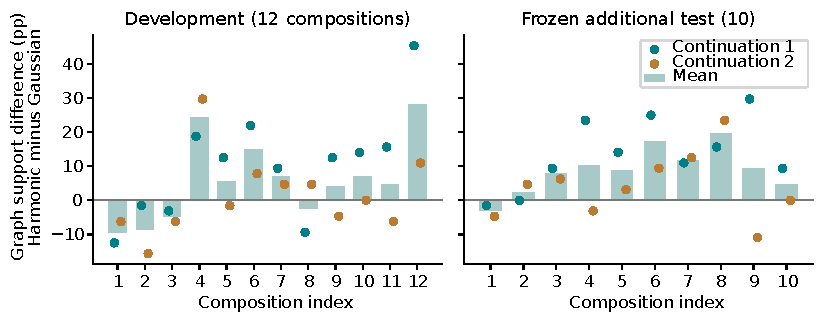
\includegraphics[width=\linewidth]{../research/figures/final_complete_v1/figures/composition_effects.pdf}
\caption{Per-composition harmonic-minus-Gaussian graph validity. Points show individual fine-tuning runs and bars their mean. Both panels use the same fitted models.}\label{fig:effects}
\end{figure}

\paragraph{Control for source covariance.}
To test whether the source benefit is explained by its covariance, we compare
against a single Gaussian with approximately the same covariance as the harmonic
mixture. We estimate that covariance from 128 trees and average over permutations
of identical atom species. An independent 8,192-tree estimate gives a relative
Frobenius error of 1.85--6.25\% across the 22 compositions. We match the training
data, optimizer, network, and sampling budgets. This follow-up compares the new
Gaussian models with the already frozen harmonic checkpoints.

\begin{table}[t]
\centering
\caption{Covariance-matched Gaussian versus harmonic source. Entries count
valid outputs over all attempts. Training and inference budgets are matched;
the Gaussian uses the calibrated covariance estimate from 128 trees.}
\begin{tabular}{llrr}
\toprule
Set & Run & Covariance Gaussian & Harmonic tree\\
\midrule
Development & 1 &332/768&436/768\\
            & 2 &313/768&388/768\\
Additional  & 1 &286/640&413/640\\
            & 2 &305/640&375/640\\
\bottomrule
\end{tabular}\label{tab:covariance}
\end{table}

Harmonic improves graph validity over this Gaussian by 11.65 percentage points
on development (paired 95\% interval [8.59,14.78]; descriptive composition interval
[8.07,15.43]) and 15.39 points on the additional set (paired [11.64,19.06];
composition [11.95,18.98]). The difference is positive in both runs on both sets.
The covariance-matched Gaussian also performs worse than the isotropic Gaussian.
These results support a benefit beyond this calibrated second-moment approximation,
consistent with a contribution from the mixture structure. The comparison adds
2,816 outputs while holding parameter count, initial self-conditioning weights,
training structures, and optimization fixed.


\section{Validity by molecular size}\label{app:wide-size}
The 64-composition panel has 16 compositions in each size stratum.
\begin{table}[t]
\centering
\caption{Raw chemical-graph validity on the 64-composition panel. Each size range
contains 1,024 attempts per method across two continuations. Values are percentages;
the final column reports percentage-point differences.}
\begin{tabular}{lrrr}
\toprule
Atoms & Gaussian & Harmonic & Difference\\
\midrule
17--28 & 49.12 & 55.08 & +5.96\\
29--40 & 24.02 & 38.28 & +14.26\\
41--52 & 16.50 & 21.29 & +4.79\\
53--64 & 9.77 & 12.40 & +2.64\\
\midrule
All 64 compositions &24.85&31.76&+6.91\\
\bottomrule
\end{tabular}\label{tab:wide}
\end{table}

\section{Additional generator evaluations}\label{app:earlier-readouts}
\subsection{An independently adapted diffusion baseline}\label{sec:edm}
We adapt the official EGNN/EDM backbone \citep{edm} to coordinate generation with atom categories fixed as conditions. Positions follow its variance-preserving schedule. Starting from the GEOM-pretrained checkpoint, each run uses the same 3,000 OMol25 references as the source-model comparison, 30,000 updates, and the original $10^{-4}$ learning rate. We evaluate the 24 new compositions using 128-call and full 1,001-call samplers, including the final observation step.

\begin{table}[t]
\centering
\caption{Raw graph validity of independently adapted conditional EDM, with 768 attempts per run. The different-backbone harmonic and force-updated models reach 52.73\% and 53.45\% at 128 calls (Table~\ref{tab:fresh-graph}).}
\begin{tabular}{lrrr}
\toprule
Sampler & Run 1 & Run 2 & Pooled rate\\
\midrule
EDM, 128 calls &103&100&13.22\%\\
EDM, 1,001 calls &93&106&12.96\%\\
\bottomrule
\end{tabular}\label{tab:edm}
\end{table}

The task and adaptation data match, but architectures and pretraining differ: EDM has 2.38 million parameters and one pass per update, versus 5.90 million and two passes for LatentSpring. EDM fine-tuning takes 481.51 and 463.61 seconds, compared with approximately 570--590 seconds for the source models. Generating 768 outputs takes 48.54/47.94 seconds at 128 calls and 377.65/374.12 seconds at 1,001 calls. Thus call counts do not equate runtime. Composition-overlap checks cover the processed OMol25 corpora only. The matched Gaussian--harmonic comparisons provide the controlled source test.

\section{Independent-backbone comparison}\label{app:matched-generators}
We train all methods from scratch on the official EDM EGNN \citep{edm}: four message-passing layers, 256 hidden features, and 2,381,566 parameters. Two independent initializations are used. Within each repetition, methods share initial weights and minibatches, with atom types fixed throughout.

\begin{table}[t]
\centering
\caption{Graph validity on 64 compositions after training from scratch on the shared 2.38-million-parameter EGNN. Each seed generates 2,048 outputs at 128 calls. The final rate pools the per-seed valid-output counts.}
\begin{tabular}{lrrr}
\toprule
Method & Valid, seed 1 & Valid, seed 2 & Pooled rate (\%)\\
\midrule
Gaussian FM & 182 & 218 & 9.77\\
Harmonic FM & 223 & 232 & 11.11\\
EDM & 301 & 216 & 12.62\\
GAGA & 321 & 249 & 13.92\\
\bottomrule
\end{tabular}\label{tab:matched-generators}
\end{table}

\paragraph{Data.}
The shared dataset contains 20,000 OMol25 training structures from 8,323 compositions and 512 internal-validation structures from 299 other compositions. All are neutral organic singlets with 8--64 atoms. Composition hashes assign the split. Selection applies contact-geometric and chemical-graph checks, without the pretrained study's scaffold filter. The 64 evaluation compositions are absent from both selected subsets and both full processed corpora.

\paragraph{Optimization.}
Each model receives 30,000 AdamW updates at learning rate $10^{-4}$ and batch size 32, totaling 960,000 training presentations. Batches have a common atom count; sampling count groups proportional to their sizes gives every row equal marginal probability. Gradients are clipped at norm one. Sampling uses the final EMA, whose decay at update $s$ is $\min(0.999,(1+s)/(10+s))$. Validation at 5,000, 15,000, and 30,000 updates monitors training without selecting checkpoints.

\paragraph{Flow matching.}
Gaussian and harmonic FM share linear interpolation, atom matching, and rotation alignment. Both use one-pass velocity prediction without self-conditioning and 64 midpoint steps, totaling 128 network evaluations. Factorized affinities permit exact tree sampling by drawing $N-2$ independent Pr\"ufer entries with probabilities $u_i/\sum_j u_j$ and decoding the sequence. This gives the same harmonic source law as the main model.

\paragraph{Diffusion.}
EDM predicts Gaussian coordinate noise under its variance-preserving schedule. Position-conditional GAGA \citep{qu2026gaga} uses the published GEOM truncation at 650 of 1,000 steps. Its starting Gaussian has variance $\alpha_t^2 v+\sigma_t^2$, where the training-only estimate $v=3.0232257866$\,\AA$^2$ is mean squared centered position per independent coordinate. The truncation is transferred from GEOM rather than selected on OMol25 evaluation results.

\paragraph{Sampling and compute.}
Each model produces 32 raw structures per evaluation composition using 128 network calls. Full EDM and GAGA schedules are also evaluated at 1,001 and 651 calls, including the observation step. No model in this comparison receives physical or bond labels, output selection, or geometry optimization. Scheduler records identify A100, H200, and A100 MIG allocations. Training presentations and call counts are matched, but runtime depends on the implementation and hardware.

\begin{table}[htbp]
\centering
\caption{Diffusion sampling at 128 calls and at the full reverse schedules. Each initialization generates 2,048 outputs; the final rate pools graph-valid counts across both initializations.}
\begin{tabular}{lrrrr}
\toprule
Method & Evaluations & Valid, seed 1 & Valid, seed 2 & Rate (\%)\\
\midrule
EDM & 128 & 301 & 216 & 12.62\\
EDM & 1,001 & 308 & 206 & 12.55\\
GAGA & 128 & 321 & 249 & 13.92\\
GAGA & 651 & 273 & 267 & 13.18\\
\bottomrule
\end{tabular}
\end{table}

\paragraph{Energy-model readout of the frozen generators.}
We score every output on the ten-composition panel and each original reference
with the same conservative eSEN checkpoint at its original charge and spin.
To retain the parity convention of the earlier oracle audit, use
$E_+(X)=[E(X)+E(-X)]/2$ and $F_+(X)=[F(X)-F(-X)]/2$.
The model measures are an energy proxy and force consistency, not independent
quantum validation. Differences are paired within composition before averaging;
energies per atom also subtract that composition's reference energy, which
cancels in the paired difference. There are 5,160 raw energy/force queries,
including both inversions of the references in each continuation's readout.
All stored inputs, outputs and derived quantities replay in the audit.

\begin{table}[t]
\centering
\caption{Harmonic minus isotropic Gaussian physical readouts on the frozen
additional panel. Lower is better for these surrogate-quality measures.
Intervals are conditional paired 95\% intervals.}
\begin{tabular}{llrr}
\toprule
Readout & Support & Difference & Interval\\
\midrule
Energy (eV/atom) & All attempts & $-0.0406$ & $[-0.0579,-0.0232]$\\
                & Common graph & $-0.0340$ & $[-0.0692,-0.0003]$\\
Force RMS (eV/\AA) & All attempts & $-0.4635$ & $[-0.6782,-0.2512]$\\
                  & Common graph & $-0.5389$ & $[-0.8950,-0.2089]$\\
\bottomrule
\end{tabular}\label{tab:physical}
\end{table}

Force RMS means the square root of the per-atom mean squared force norm,
then averaged over samples. The common-graph statistic uses only paired outputs
accepted by both methods; cell counts range from 3 to 35. It is a
selected-support estimand and is not an unbiased equilibrium expectation.
All-attempt statistics include outputs rejected by the structural assay and may
reflect potential-model extrapolation. The two readouts therefore answer different
questions and are both retained. Their positive direction strengthens the quality
interpretation of the source result, but lower energy or force magnitude does not
establish a Boltzmann distribution or remove the need for independent physical
validation.

Continuation effects are heterogeneous. All-attempt energy differences are
$-0.08049$ and $-0.00070$ eV/atom; force-RMS differences are $-1.21996$ and
$+0.29302$ eV/\AA. Thus the pooled force advantage does not replicate in sign
across both continuations, and the second energy effect is small. The conditional
intervals do not quantify uncertainty over independently retrained models.

\paragraph{Original endpoint checkpoint.}
The original 30,000-step OMol25 checkpoint generates coordinates from fixed composition and neutral/no-bond inputs using a bootstrap step followed by 127 Euler updates. At 128 calls, retaining predicted categorical history gives 106/640 and 113/640 graph-valid outputs in two sampling streams. Fixing history categories and centering the bootstrap gives 116/640 and 120/640. Both streams share the checkpoint, and the second configuration changes both history and centering. LatentSpring source models additionally receive shared task adaptation and 3,000 specialized updates; their matched Gaussian and covariance-Gaussian variants isolate source choice.

\section{Normalization of the harmonic mixture}\label{app:proof}
For a tree $T$, let $B_T\in\RR^{(N-1)\times N}$ be its edge-incidence matrix, with one row per edge and entries $+1$ and $-1$
at the edge's two endpoints. Let $U\in\RR^{N\times(N-1)}$ have orthonormal columns spanning the centered subspace.
Because $B_T\mathbf1=0$, $(B_TU)(B_TU)^\top=B_TB_T^\top$. Cauchy--Binet expresses
$\det(B_TB_T^\top)$ as the sum of squares of its $N$ maximal minors. Each minor
of a tree incidence matrix is $\pm1$, so the determinant is $N$. The absolute
Jacobian in one spatial dimension is therefore $\sqrt N$, and in three dimensions
it is $N^{3/2}$. Consequently the component density is
$q(X\mid T,c)=N^{3/2}\prod_{e\in T}h_e(B_TX)$ and integrates to one. Averaging
with Equation~\eqref{eq:tree-law} yields Equation~\eqref{eq:source} and preserves
normalization.

\section{Source invariance under symmetry coupling}\label{app:symmetry}
Let $G$ be the compact group of proper rotations and permutations of identical
conditioning labels. Suppose $q_0$ is $G$-invariant, $X\sim q_0$, and a pairing
algorithm selects $g(X,Y)\in G$ using a target $Y$. If $H$ is an independent Haar
draw, then conditional on the orbit of $X$ and on the selected $g$, $HgX$ has
the uniform orbit distribution of $HX$, by Haar invariance. Integrating over the
unchanged source-orbit distribution recovers $q_0$. This argument permits a
non-Gaussian source and explains the shared augmentation used in the pairing.
The paired endpoints remain correlated; our training objective uses their
conditional displacement target directly.

\section{Covariance controls}
The shell control draws a positive edge length $R$ concentrated around the
radius-based scale $\ell$, then chooses its direction uniformly. Specifically,
$R=\ell\exp(sZ-s^2/2)$, where $Z\sim N(0,1)$ is a scalar standard Gaussian and
$s=0.2$ controls the spread of log lengths. Its second moment is
$\EE R^2=\ell^2\exp(s^2)$.
A uniform direction has second moment $I/3$, so each edge has covariance
$vI=\ell^2\exp(s^2)I/3$. Let $A_T$ map edge coordinates to centered node
coordinates. Independence gives $C_T=A_T\operatorname{diag}(v_e)A_T^\top$.
Here $C_T$ describes correlations between atom positions for a fixed tree,
and $\operatorname{diag}(v_e)$ places its edge variances on a diagonal matrix.
Replacing the edge vectors by independent Gaussians of covariance $v_eI$ leaves
$C_T$ unchanged and, since all component means are zero, leaves $\EE_TC_T$
unchanged. The single-Gaussian control uses a finite, composition-seeded average
of these matrices. Averaging this matrix over within-species permutations preserves
positive definiteness on the centered subspace and yields species invariance.
The Gaussian is exactly normalized for its chosen covariance; equality to the
infinite tree-mixture covariance remains approximate.

\section{Jarzynski identity for escorted transport}\label{app:jarzynski}
Jarzynski's relation connects exponential work averages with equilibrium
free-energy differences, including in single-molecule pulling experiments
\citep{jarzynski1997master,hummerszabo2001}. Escorted transport introduces an
imposed flow and includes its configuration-volume correction in the work
\citep{escorted2008}. The change-of-variables form provides the basis for our
local-reference construction.

Fix a composition and measure volume within its centered coordinate space.
In this subsection, $x$ denotes all independent coordinates of a molecule.
Write $\beta=1/(k_B T_{\rm phys})$ for inverse thermal energy. The function
$\rho_1(x)=\mathbf1_\Omega(x)\exp[-\beta E(x)]$ defines an unnormalized
target density with finite, nonzero
$Z_1=\int_{\HH_N}\rho_1(x)\,dx$, for example a declared confined molecular ensemble.
The indicator $\mathbf1_\Omega$ equals one inside the allowed configuration region
$\Omega$ and zero outside it. Restricting this region makes the integral finite.
Dividing $\rho_1$ by $Z_1$ gives the target probability density.
Let $q_0>0$ be the normalized source in Equation~\eqref{eq:source}, and let
$\Phi:\HH_N\to\HH_N$ be a differentiable bijection with nonzero intrinsic Jacobian.
Here $\Phi$ is an imposed, invertible transformation of coordinates. Its Jacobian
matrix $D\Phi$ contains the derivatives of output coordinates with respect to
input coordinates; the absolute determinant measures local expansion or compression.
For $\Phi(x_0)\in\Omega$, define the generalized work
\begin{equation}
 W_\Phi(x_0)=E(\Phi(x_0))+
 \beta^{-1}\log q_0(x_0)-
 \beta^{-1}\log|\det D\Phi(x_0)|,
\end{equation}
and set $W_\Phi=+\infty$ otherwise, assigning zero weight to an inadmissible
configuration. Then
\begin{align}
 \EE_{q_0}[e^{-\beta W_\Phi}]
 &=\int_{\HH_N}\rho_1(\Phi(x_0))|\det D\Phi(x_0)|\,dx_0\\
 &=Z_1.
\end{align}
Equivalently, the auxiliary source energy $E_0=-\beta^{-1}\log q_0$ has $Z_0=1$
in the declared measure, yielding a Jarzynski-type normalizer identity.
The Jacobian term accounts for compression by the escort map. For an observable
$f$, such as energy or a function of a rotation angle, target averages are estimated
by $\sum_j w_j f(\Phi(x_j))/\sum_j w_j$, where $w_j=e^{-\beta W_\Phi(x_j)}$.
This is self-normalized importance sampling: each transformed sample contributes
according to its corrected weight. Finite-sample variance depends on how well
the proposals cover the target distribution.

For an exact, sufficiently regular ordinary differential equation (ODE) flow,
the intrinsic log determinant is the integral of the velocity divergence, which
sums the local rates of expansion of independent coordinate directions.
Our implementation makes the work tractable
through explicit local references: translations of Gaussian anchor distributions
in Appendix~\ref{app:local-work}, and periodic rotor maps with analytic Jacobians
in Appendix~\ref{app:rotor-work}. The neural generator itself is evaluated through
its raw samples, using the midpoint solver and terminal noise specified in
Section~\ref{sec:flow}.

\section{Local force-escorted work distillation}\label{app:local-work}
The physical teacher combines local force-guided proposals with energy-weighted
flow matching \citep{dern2025energyweighted,fab}. Normalized anchor references
make the escorted-work weights explicit \citep{escorted2008}.

\paragraph{Energy, force and mirror symmetry.}
The energy model assigns a scalar $E(X)$ to a geometry and provides its force
$F(X)=-\nabla_X E(X)$, a vector for each atom. The force points in the direction
of decreasing energy. We average a geometry and its inversion through the origin:
$E_+(X)=[E(X)+E(-X)]/2$ and $F_+(X)=[F(X)-F(-X)]/2$.
The opposite sign in the force average preserves $F_+=-\nabla E_+$.
This construction assigns equal energy to mirror-related geometries and opposite
forces to their inverted coordinates. We remove the mean atom force before
constructing displacements, keeping them in the centered coordinate space.

\paragraph{Local reference and target.}
For a generated training anchor $A$ with accepted perceived graph $G_A$, define
$q_A(X)=\mathcal N_{\HH_N}(A,\sigma_A^2I)$.
Write $kT=k_B T_{\rm phys}=0.0258519998$ eV for the thermal energy at 300 K.
We set
\begin{equation}
 \sigma_A=\min\left(0.03\,\text{\AA},
 \sqrt{\frac{0.10\,\text{\AA}\,kT}{\|F_+(A)\|}}\right),\qquad
 \delta_A=\frac{\sigma_A^2}{kT}F_+(A).
\end{equation}
A vanishing force selects the maximal width. The force norm is the Frobenius
norm over all atom-force components. These choices bound that same norm of the
displacement by $0.10$\,\AA\ and the Gaussian width by $0.03$\,\AA.
These quantities are fixed before
drawing $X\sim q_A$. The escort $Y=X+\delta_A$ is a translation on the centered
subspace and has determinant one. The local unnormalized target is
\begin{equation}
 \rho_A(Y)=q_A(Y)\exp\!\left[-\frac{E_+(Y)-E_+(A)}{kT}\right]
 \mathbf1_{G_A}(Y),
\end{equation}
where the support requires the same labelled perceived bond orders, formal charges
and radical counts, together with the connected/nonoverlap assay. The graph is
inferred from the anchor coordinates. The resulting target is a local energy tilt
restrained around $A$ by $q_A$.

\paragraph{Why the force displacement has this form.}
Locally approximate the molecular energy by its value and force at the anchor:
$E_+(Y)-E_+(A)\simeq-\langle F_+(A),Y-A\rangle_F$, where the inner product sums
force times displacement over every atom and coordinate. Completing the square
in the Gaussian gives
\begin{equation}
 q_A(Y)\exp\!\left[\frac{\langle F_+(A),Y-A\rangle_F}{kT}\right]
 \ \propto\
 \mathcal N_{\HH_N}\!\left(Y;A+\frac{\sigma_A^2}{kT}F_+(A),\sigma_A^2I\right).
 \label{eq:linear-boltzmann-escort}
\end{equation}
Thus the force escort samples the local Boltzmann tilt exactly for a linearized
energy, before applying the same-graph restriction. The Gaussian restraint acts
like a virtual harmonic spring with stiffness $kT/\sigma_A^2$: the force shifts
its mean by force divided by stiffness. This explains the displacement scale.
The graph restriction subsequently truncates this local distribution.

\paragraph{Complete local work.}
With reference Hamiltonian $H_0=-kT\log q_A$ and target Hamiltonian
$H_1=H_0+E_+-E_+(A)$ plus hard support, the generalized quench work is
\begin{equation}
 W_A(X)=E_+(Y)-E_+(A)+kT[\log q_A(X)-\log q_A(Y)]
\end{equation}
on valid support, and $+\infty$ otherwise. Change of variables gives
$\mathbb E_{q_A}[\exp(-W_A/kT)]=\int\rho_A(Y)\,dY$.
The two reference-density terms correct for the escort's proposal shift.
Analytic checks recover constant work for a constant-force escort and the
normalizer and weighted mean for a quadratic energy.
For the linearized energy in Equation~\eqref{eq:linear-boltzmann-escort},
substitution gives the same work
$W_A=-\sigma_A^2\|F_+(A)\|_F^2/(2kT)$ for every supported candidate.
Uniform weights are therefore appropriate in this approximation. Complete-work
weights use the actual nonlinear energy to correct deviations from it. This
distinguishes the inexpensive force-only teacher from its energy-weighted extension.

\paragraph{Training and controls.}
Each continuation selects eight distinct 17--28-atom training compositions by a
fixed metadata hash and generates 32 anchors per composition. These compositions
are disjoint from evaluation. Invalid anchors remain in the generation counts
and are excluded from the teacher pool. Each valid anchor produces eight escorted particles. Particles outside
its declared support receive zero weight. The work arm samples training endpoints
using self-normalized $\exp(-W_A/kT)$ weights; the unweighted escort arm samples the
same valid particles uniformly. A replay arm uses the retained raw anchors, and a
frozen model supplies the reference. All-zero-particle anchors are recorded and
excluded identically from all student pools.

Each student alternates 500 original-reference FM updates with 500 generated-anchor
endpoint updates, sharing initialization, anchor draws, optimization and sampling
budgets. Physical preparation costs differ: replay needs no force queries, the
unweighted escort needs anchor forces, and complete work additionally needs
energies at valid proposed endpoints. Actual shared research cost and these
method requirements are reported separately. The final generator uses the
learned network alone. Its temperature feature stays fixed throughout training
and evaluation; 300 K determines the local teacher weights. Self-normalization
introduces finite-particle bias, and the reported teacher ESS is computed over
the eight local particles at each anchor.
Effective sample size (ESS) is $(\sum_j w_j)^2/\sum_j w_j^2$ for candidate weights
$w_j$. It equals the candidate count for equal weights and approaches one when
a single candidate dominates.

\paragraph{Direct fine-tuning results.}
We train three students for 1,000 updates in each run. Across 512 generated
anchors, 351 pass the graph checks and 349 have at least one allowed force-shifted
candidate. Composition-level mean ESS is about 1.27--1.87 out of 8. The weights
are therefore concentrated on few candidates, limiting resolution of the local
target with this pool size.

\begin{table}[t]
\centering
\caption{Graph-valid outputs after direct physical fine-tuning, out of 640
attempts per run. The frozen model receives no updates; all other variants have
the same additional training budget.}
\begin{tabular}{lrrrr}
\toprule
Run & Frozen & Replay & Unweighted escort & Complete work\\
\midrule
1 &418&340&330&344\\
2 &377&345&371&362\\
\bottomrule
\end{tabular}\label{tab:local-work-direct}
\end{table}

Among paired outputs that are both graph-valid, complete-work training gives
lower energy than unweighted-escort training by 0.00758 eV/atom (paired 95\%
interval $[-0.01424,-0.00113]$ for the signed difference). Force RMS is lower by
0.16174 eV/\AA\ ($[-0.27660,-0.05590]$). Both runs favor complete work, and
the all-output comparison has the same direction.

However, all three directly fine-tuned students perform worse than the frozen
model. Complete work has 55.16\% graph validity versus 62.11\% for the frozen
model, and energy on paired, jointly valid outputs is \emph{higher} by
0.10587 eV/atom ($[0.09009,0.12168]$). Replay also worsens performance after
training on the mixed targets. These results motivate subtracting the matched
replay update rather than using the physical student directly.

Teacher preparation uses 6,232 raw energy/force queries: 702 at anchors and
5,530 at allowed candidates. The unweighted escort could omit candidate-energy
queries, and replay could omit all physical queries. Scoring the outputs of the
four models uses a further 10,240 queries, separate from generation cost.


\paragraph{Applying the paired physical update.}
Instead of deploying the directly fine-tuned student, we use parameter arithmetic
\citep{ilharco2023arithmetic} to subtract its matched replay update:
\begin{equation}
 \theta_{\rm final}=\theta_{\rm base}
   +(\theta_{\rm physical}-\theta_{\rm replay}),
\end{equation}
for both unweighted-escort and complete-work students. The coefficient is fixed
at one. We change parameter tensors only; buffers and the source distribution
remain fixed.

\begin{table}[t]
\centering
\caption{Paired updates evaluated after the direct fine-tuning experiment.
Energy changes use paired, jointly valid outputs and are relative to the frozen
model, with paired 95\% confidence intervals. Counts show the two generation
streams.}
\begin{tabular}{lrr}
\toprule
Model & Graph-valid outputs (two streams) & Energy change (eV/atom)\\
\midrule
Frozen &418/640; 377/640&$0$\\
Paired force update &407/640; 387/640&$-0.01554\;[-0.02084,-0.01031]$\\
Paired work update &406/640; 382/640&$-0.01604\;[-0.02188,-0.01013]$\\
\bottomrule
\end{tabular}\label{tab:thermal-transfer}
\end{table}

Both paired variants lower energy and force RMS in both runs. For complete work,
force RMS on paired, jointly valid outputs falls by 0.38403 eV/\AA\ (interval
$[-0.48124,-0.28932]$); all-attempt energy and force scores also improve. Its
graph-validity difference from the frozen model is $-0.55$ percentage points,
with interval $[-2.58,1.56]$.

The complete-work and unweighted paired variants have similar scores. Complete
work minus unweighted gives $-0.00243$ eV/atom on jointly valid pairs
($[-0.00756,0.00264]$) and $+0.00022$ eV/atom over all attempts
($[-0.00557,0.00649]$). Force and graph-validity intervals also include zero.
Teacher preparation requires 702 anchor queries for the unweighted variant
versus 6,232 for complete work. Both retain the 128-call neural sampler.

Evaluating these two paired variants adds 2,560 generated outputs and 5,120
physical queries. Combining parameters requires no optimizer steps. Based on
these development results, we select the force-only update for the
new-composition evaluation in Section~\ref{sec:fresh-physics}.



\section{Molecular rotor work protocol}\label{app:rotor-work}
We test the work correction on three controlled methyl rotations: \texttt{C=C(N)N(C)C(N)=O}, \texttt{CCOC(C)(C)N}, and \texttt{CC(=O)NCC=O}. Among the first five rows of an existing training subset, we select the first three distinct compositions whose rotor preserves the inferred labeled graph on a 64-angle grid. Selection uses geometry alone. Only methyl hydrogens rotate around the carbon--anchor axis; other internal coordinates remain fixed. We remove translation and define densities with respect to $d\phi$ on $[-\pi,\pi)$.

\paragraph{Reference and map.}
The circular reference is $q_0(\phi)=\exp(\cos\phi)/(2\pi I_0(1))$, with $2\pi I_0(1)=\int_{-\pi}^{\pi}\exp(\cos u)\,du$. Its Hamiltonian is $H_0=-kT\log q_0$, and the target is defined by $H_1=H_0+U-U(0)$. For $a\in\{-0.5,0,0.5\}$, the map $\psi_a(\phi)=\phi+a\sin\phi$ has Jacobian $J_a(\phi)=1+a\cos\phi$. Because $|a|<1$, it is smooth and invertible on the circle. Complete work is
\begin{equation}
 W_a(\phi)=U(\psi_a(\phi))-U(0)+kT\left[
 \log q_0(\phi)-\log q_0(\psi_a(\phi))-\log J_a(\phi)\right].
\end{equation}
The reference-density and Jacobian terms correct changes in angular sampling and interval volume. Changing variables gives
\begin{equation}
 \EE_{q_0}e^{-W_a/kT}
 =\int_{-\pi}^{\pi}q_0(y)e^{-[U(y)-U(0)]/kT}\,dy=Z_1/Z_0,
 \qquad Z_0=1.
\end{equation}

\paragraph{Numerical reference.}
All 1,536 GFN2 single-point calculations succeed. Each rotor energy curve uses a periodic cubic interpolation of 512 values. At the added midpoint samples, the 256-knot interpolation differs by at most $10^{-8}$ eV. Doubling quadrature resolution from 32,768 to 65,536 changes free energy by less than $10^{-10}$ eV.

\paragraph{Estimators.}
Total variation uses 64 equal angular bins with quadrature-based target probabilities. The mean unnormalized weight is unbiased for the normalizer, whereas self-normalized observable estimates have finite-sample bias. Free-energy RMSE for $-kT\log\widehat Z$ includes its finite-sample bias. At 2,048 draws, complete-work ESS ranges from 788 to 1,892 across six nonidentity cases. Incomplete weights can have higher ESS while targeting an incorrect distribution, so distribution error is evaluated separately.


\end{document}
